\subsubsection{Scalability, performance and constraints} \label{section:scalability}

\paragraph{Availability and downtime}
Some client-server systems are very vulnerable to server breakdowns, as they, in many cases, drastically reduce service's bandwidth, or make the service stop working altogether. High availability and low downtime is a must for a highly congested client-server architecture. These factors are strongly dependent on the server infrastructure, its degree of decentralization, integration of data migration tools and possesion of back-up servers. Ethereum, however, possesses high degree of availability, due to its decentralized nature. If one of the nodes fail, there are still plenty of other nodes available.

\paragraph{Unpredicted confirmation delay}
When dealing with blockchain based systems, it is important to consider that a newly generated transaction has to be added to a block, before being confirmed and validated. This process may take different amounts of time, depending on the network's current state and network's target block time. Ethereum's target block time of 15 seconds is quite short, comparing to other blockchains like ZCash and Bitcoin, whose block times are 2.5 and 10 minutes respectively. However, even if a transaction is included into the blockchain's next block by the miners, the data will not become a part of the blockchain until the block has been mined. Target block time does not provide any guarantee that the block will be added to the chain within the target time, as the mining process itself involves a degree of randomness. Thus, the block finding time is heavily dependent on luck factor and is impossible to predict. A test, in which actual block times of 10000 blocks of Ethereum are analyzed can be found in Figure \ref{fig:ethtimetest} of Appendix \ref{section:blocktimes}.

There is as well no guarantee on the number of new blocks being found before the generated transaction itself will be included into a new block. This is heavily dependent on the gas price, which is chosen for the transaction. In applications that need to perform a large number of smart contract function calls, there is a trade-off to be made between the cost and latency, as faster response times will be a lot more expensive to achieve (detailed discussion about that is provided in \ref{section:economics}).

Introduction of such delay makes the implementation of applications, in which the responsiveness is a key factor, impossible. Such example is applications for real time monitoring. In some systems it is crucial to be notified about a problem, or a system state change as soon as possible. By using Ethereum to power such application, operators in the control room would not be notified about, for example, a potential problem which generates an alarm, before the transaction, that was generated by the alarm contract, was mined (which, as explained before can be take indefinite amount time). In such systems it is much more viable to use client-server architecture-based alarm system.

\paragraph{Ethereum's throughput and scalability} 
One of the main things to consider, when talking about a system's performance, is its maximum throughput and how it can be increased when needed. In Ethereum, the maximum throughput of the network is defined by the gas limit of the blocks and their frequency, using the following formula:

\begin{equation} \label{eq:eththroughput}
T_{\mathrm{net}} = \frac{1}{t_b} \cdot L_b = \frac{L_b}{t_b}
\end{equation}

Ethereum's block time $t_b$ is equal to 15 seconds, which can be converted to 1/240 hours. Block gas limit is equal to $8 \cdot 10^6$ at the time of writing. This block gas limit $L_b$ can be changed by miners, depending on overall network hashrate and congestion. Thus, by inserting the values into Equation (\ref{eq:eththroughput}), the current total throughput rate of Ethereum, $T_{\mathrm{net}}$, is approximately $1.6 \cdot 10^9$ gas/hour.

A basic Ethereum transaction for token transfer consumes 21000 gas, thus the current theoretical transaction capacity of Ethereum is approximately 76200 tx/h, assuming that none of the contracts executes any code. The theoretical transaction capacity is significantly reduced, when introducing transactions that require computational effort. 

The block gas limit has historically been increasing as a result of the growing hashrate of Ethereum network. The main reason for the existence of gas limit is to enable consensus participation of smaller mining nodes, thus further decentralizing the network. All of the transactions and their associated code has to be verified by the nodes. So without a proper limit on amount of gas per block, the nodes could potentially be overwhelmed. 

As mentioned earlier, increased congestion of the network can be addressed by adjusting the block gas limit $L_b$. The result of that gas limit would lead to a proportional increase in throughput in terms of gas, according to Equation (\ref{eq:eththroughput}).

\begin{figure}[H]
\centering
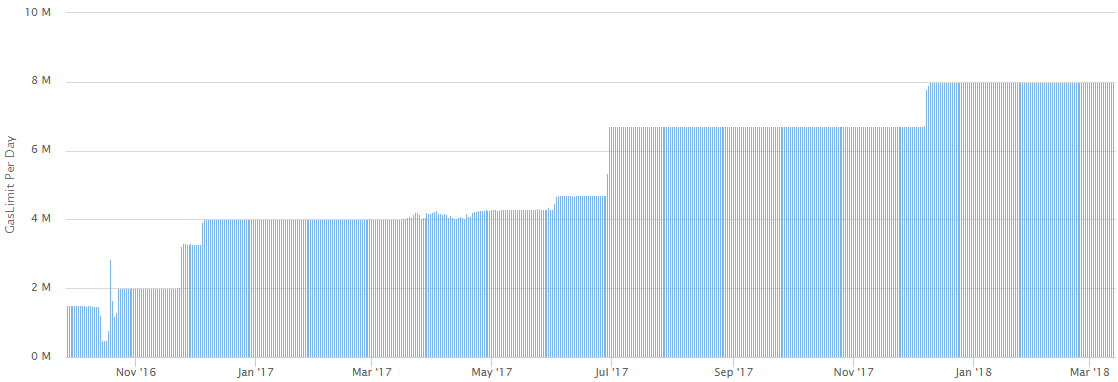
\includegraphics[scale=0.49]{images/gasblocklimit.png}
\caption{Gas block limit increase. Limit has been increased by four times since October 2016 to accommodate the growing congestion \textnormal{\citep{ethgaslimit}}.}
\label{fig:ethergasblocklimit}
\end{figure}

Nevertheless, despite the throughput's flexibility, which is provided by the gas block limit adjustment, it would be wrong to say that Ethereum possesses good scalability, as its theoretical average throughput of around 21 transactions per second is extremely poor, in comparison to typical client-server systems. The throughput needs to be scaled by an extremely large factor, in order for Ethereum network to possess comparable throughput to a typical client-server system, which can not be achieved fast enough by just increasing the gas block limit alone. 

\paragraph{Storage and memory}
Each and every smart contract has its own independent storage. That storage is virtual and is structured in terms of indexable key-value pairs. There are $2^{256}$ key-value pairs in each contract, with each pair having a capacity of storing 32 byte words, that results in a storage capacity of $2^{261}$ bytes. Thus, there is no doubt that there is plenty of storage, which is an understatement (as it turns out, a single smart contract has a theoretical capacity to store all of the humanity's data billions and billions times over).

This all sounds really good on paper, however, there is a cost that comes with using this storage. Storing a single 256-bit word consumes 20000 gas ({\small SSTORE} operation when the value is altered from zero to non-zero), excluding the base transaction cost of 21000 gas. In order to upload large files to smart contracts, they would need to be broken down to small 256-bit chunks and stored in different key-value pairs, using {\small SSTORE}. Equation (\ref{eq:filestorage}) derives the cost of storing a file in a smart contract.

\begin{align} \label{eq:filestorage}
C_{\mathrm{store}} = C_{\mathrm{gas}}\left(\frac{Q \cdot G_{sstore}}{256} + G_{tx}\right) \cdot 10^{-9} \cdot C_{ETH}  
\end{align}

Here, $Q$ is the file size. The file size is given in megabytes (1 megabyte is equal to $8 \cdot 10^6$ bits). Gas consumption of a single {\small SSTORE} operation, $G_{\mathrm{sstore}}$, is 20000. Base transaction cost, $G_{\mathrm{tx}}$, is 21000. Assuming that a gas price, $C_{\mathrm{gas}}$, of 2 Gwei was used, the following equation is derived.

\begin{align}
C_{\mathrm{store}} &= 2 \cdot \left(\frac{8 \cdot 10^6 \cdot 20000 \cdot Q}{256} + 21000\right) \cdot 10^{-9} \cdot C_{ETH} \approx 1.25 \cdot C_{ETH} \cdot Q
\end{align}

Thus, a single megabyte of storage costs approximately 1.25 ETH, or 875 USD! That is an exceptionally high price to pay, considering that services like Dropbox offer cloud storage of 2 terabytes at a monthly cost of around 12 USD \citep{dropbox}.

Another limitation on storage of large files in smart contracts is the gas block limit $L_b$. A transaction may obviously not exceed the gas block limit, as it would be impossible for it to be included in a block otherwise. Considering the current block gas limit of $8 \cdot 10^6$, the theoretical maximum amount of {\small SSTORE} operations triggered within a single transaction is derived using following equation.

\begin{align}
N_{sstore} = \floor[\Bigg]{\frac{\left(L_b - G_{tx} \right)}{G_{sstore}}} = \floor[\Bigg]{\frac{\left(8 \cdot 10^6 - 21000\right)}{20000}} = 389
\end{align}

Thus, there will be an overhead of 21000 gas approximately each 389 {\small SSTORE} operations (which corresponds to storage of 99584 bits). Equation (\ref{eq:filestorage}) needs to be modified with that overhead in mind.

\begin{align} \label{eq:newstorecost}
C_{\mathrm{store}} = C_{\mathrm{gas}}\left(\frac{Q \cdot G_{sstore}}{256} + G_{tx}\left(\frac{Q}{256}\middle/\floor[\Bigg]{\frac{\left(L_b - G_{tx} \right)}{G_{sstore}}}\right)\right) \cdot 10^{-9} \cdot C_{ETH} 
\end{align}

By numerically solving (\ref{eq:newstorecost}), the cost of storage turns out to be equal to approximately 1.266 ETH, or 886.20 USD$^\star$ per megabyte.

Additional consequence of splitting the file storage process into multiple transactions, spanning multiple blocks, is that the upload might take a long time, as the target block time is around 15 seconds. Assuming that each and every following block is filled with file content upload transactions until the storage process is completed, the average transmission speed would be 99.6 kilobits every 15 seconds, which translates into roughly 6.6 kilobits second. Even the dial up modems from the 90s had faster speeds of around 56 kilobits per second \citep{dialup}. At that rate the storage process of one megabyte would span over 81 blocks, thus taking approximately 20.25 minutes to complete, assuming that no other transactions are being included in any of those 81 blocks (but the last one), which is very unlikely.

However, once the data is added to the smart contract's storage it is free to access, using \texttt{get()} methods.

\paragraph{Scalability and performance of centralized systems}
Systems that are using a client-server architecture are relying heavily on the servers, when dealing with increased amount of traffic. There are countless server solutions, which sparks a competition among server providers. This competition drives the technology forward, thus making single server units being able to handle more and more traffic.

Servers are typically located in server racks inside of big data centers. The process of adding additional server units to accommodate the increased amount of traffic is typically as easy as stacking more units on top of eachother on a server rack. Increased storage demands can be addressed by upgrading existing storage disks to larger capacities, or just adding more of them. However, this can sometimes require some maintenance downtime.

\paragraph{Choice of key sizes}
As mentioned before in this section, extensive computation complexity and large requirements on storage of the smart contracts leads to extremely high gas consumptions. That is why it is very important to go as far as optimizing each and every variable in the smart contract code as it would significantly reduce gas consumption of execution and contract deployment. For optimization purposes, ECDSA 256-bit keys are used in Ethereum, as well as many other blockchains. The reason for that is the rather short key size, which is beneficial in terms of gas and computational effort savings.

One of the most common asymmetric cryptographic algorithms, RSA, which is used in many centralized applications, typically uses 1024- and 2048-bit keys for encryption, which is considerably larger then then 256-bit keys in ECDSA cryptography in Ethereum. The reason for that is that ECDSA is more cryptographically complex than RSA, as was described in \ref{section:analysisencryption}, which leads to smaller key sizes needed.

\paragraph{Symmetric key cryptography and public blockchains}
As mentioned in \ref{section:analysisencryption}, transmission of private keys on the blockchain is a really bad idea due to its transparency. Thus, symmetric encryption algorithms, such as AES and DES, can not be implemented on Ethereum, as the secret key would be visible to everyone on the network, making it rather useless. This is obviously not the case in the centralized systems as long as a secure communication channel is established.

\paragraph{Implementation constraints}
Blockchain is a relatively new technology. At the time of writing, there are only a few blockchains that support smart contract scripting functionality. Smart contracts are written in contract-oriented programming languages, out of which Solidity is the superior one. Solidity is considered being quite low-level to make it easier to optimize code, as storage and instruction executions are quite expensive in Ethereum. Solidity is also highly criticized for some of it's design flaws, such as static 256-bit word lengths, confusing type names (for example, \texttt{bytes32} is a byte array that has a size of 256 bits and \texttt{uint32} is an integer that has a size of 32 bits, which can be very confusing), no string manipulation support, no null pointer support, no floating point numbers and so on \citep{soliditybad}. 

When developing non-blockchain applications, there is a great choice of different design patterns that can be used for development, as well as a wide selection of available programming languages for all needs. This gives programmers a lot more freedom during the implementation and system design phase. The freedom of implementation approaches is strongly dependent on the type of application being implemented. The point is that the range of possible applications that can be built on a client-server architecture is significantly larger than the range of applications that can be built on Ethereum.


